\documentclass{article}
\usepackage{tipa}
\usepackage{graphicx, cleveref}

\title{Audio Analysis}
\author{Zhean Ganituen}
\begin{document}
\maketitle

\section{Pronunciation of ``Halo-Halo''}

The Filipino dessert \emph{Halo-Halo} is often mispronounced, largely due to
differences between Tagalog and English orthography. The name is also
frequently confused with the common Tagalog expression \emph{halo-halo}
(``mixed together'').\footnote{English translation: \emph{mixed together}. For
    example, ``\emph{Pinag-halo-halo ang mga estudyante sa iba't ibang seksyon}'':
    ``The students were \emph{mixed together} into different sections.''}

The literal pronunciation of the Filipino word ``halo-halo'' is a reduplication
of the lexeme ``halo'' as /\textipa{halo}/ or /\textipa{hal'o}/, with a glottal
stop occurring between the alveolar lateral approximant [\textipa{l}] and the
close-mid back rounded vowel [\textipa{o}]. Another variant is the
reduplication of the phoneme ``halu'' as /\textipa{halu}/ or /\textipa{hal'u}/.

For brevity, we will use ``\emph{Halo-Halo}'' to refer to the dessert, and
``\emph{halo-halo}'' to refer to the adjectival or verbal expression.

\subsection{Mispronunciations of ``Halo-Halo''}

Figure~\ref{fig:halo} illustrates the spectrogram corresponding to each
mispronunciation of ``Halo-Halo''.

\paragraph{Reduplication of /\textipa{halo}/} The spectrogram in
\Cref{fig:halo} shows a continuous and repeating speech pattern.

\begin{figure}
    \centering
    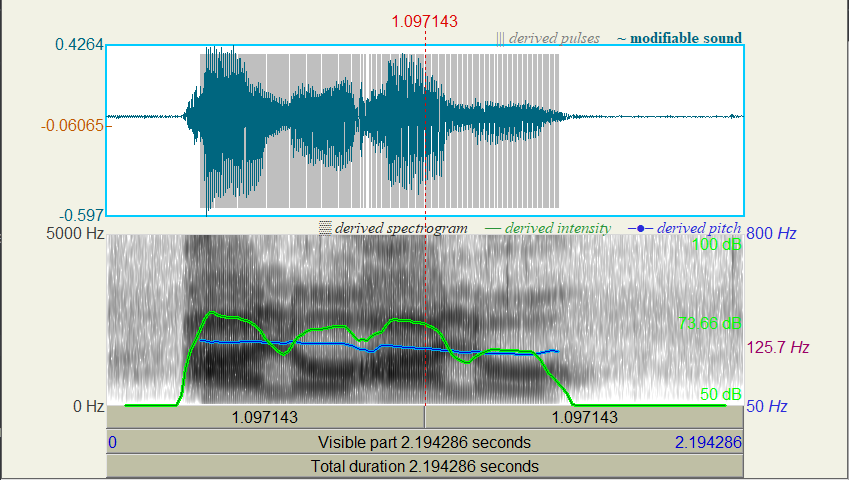
\includegraphics[width=0.65\linewidth]{img/halo.png}
    \caption{Reduplication of /\textipa{halo}/}\label{fig:halo}
\end{figure}

\paragraph{Reduplication of /\textipa{hal'o}/} \Cref{fig:hal'o} shows repetitive speech pattern with
an abrupt stop in between each root word due to the glottal stop /\textipa{l'o}/. In fact, this is the
correct pronunciation of ``halo-halo''.

\begin{figure}
    \centering
    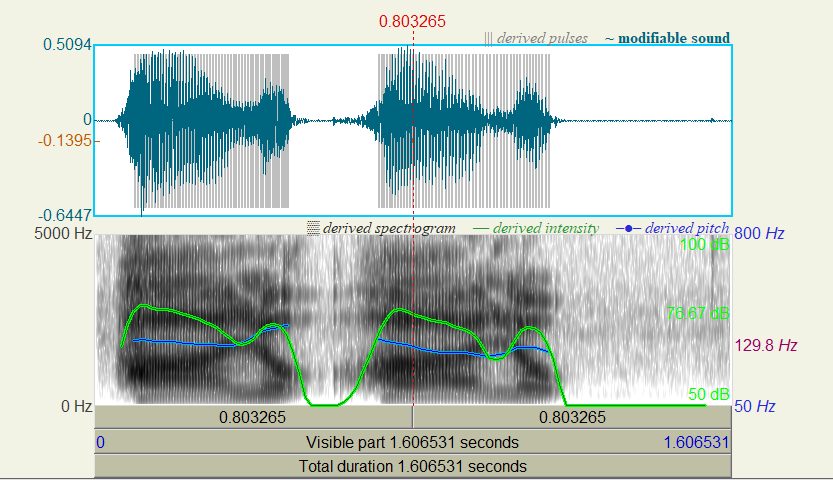
\includegraphics[width=0.65\linewidth]{img/hal_o.png}
    \caption{Reduplication of /\textipa{hal'o}/}\label{fig:hal'o}
\end{figure}

\paragraph{Reduplication of /\textipa{halu}/} \Cref{fig:halu} shows continuous and repeating
speech pattern.

\begin{figure}
    \centering
    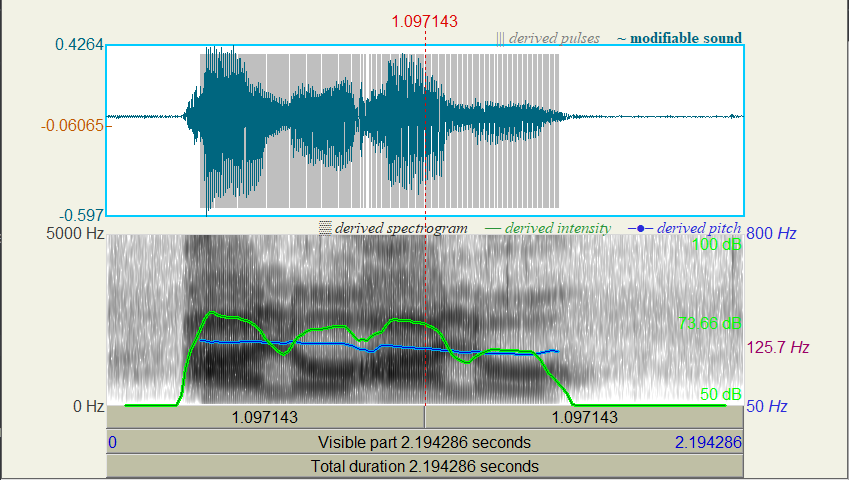
\includegraphics[width=0.65\linewidth]{img/halo.png}
    \caption{Reduplication of /\textipa{halu}/}\label{fig:halu}
\end{figure}

\paragraph{Reduplication of /\textipa{hal'u}/} \Cref{fig:hal'u} shows repetitive speech pattern with
an abrupt stop in between each root word due to the glottal stop /\textipa{l'u}/.

\begin{figure}
    \centering
    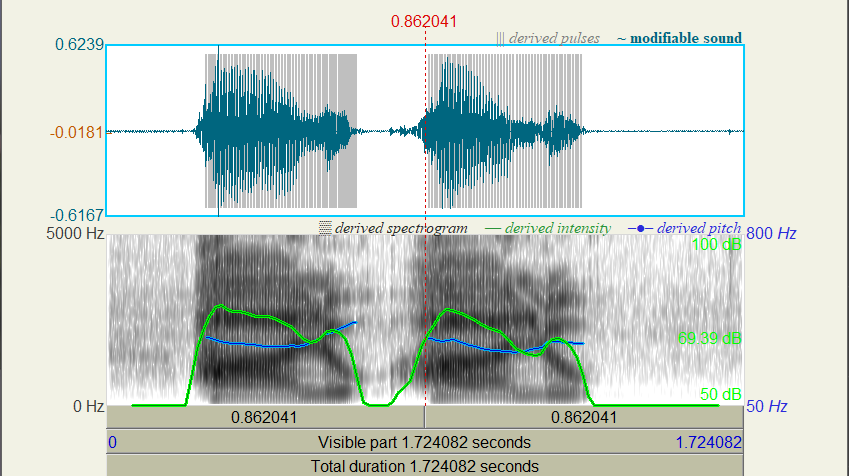
\includegraphics[width=0.65\linewidth]{img/hal_u.png}
    \caption{Reduplication of /\textipa{hal'u}/}\label{fig:hal'u}
\end{figure}

We also see the differences between the /\textipa{u}/ and the /\textipa{o}/
sound in the spectrogram as /\textipa{u}/ tends to have a lower frequency than
/\textipa{o}/.

\begin{figure}
    \centering
    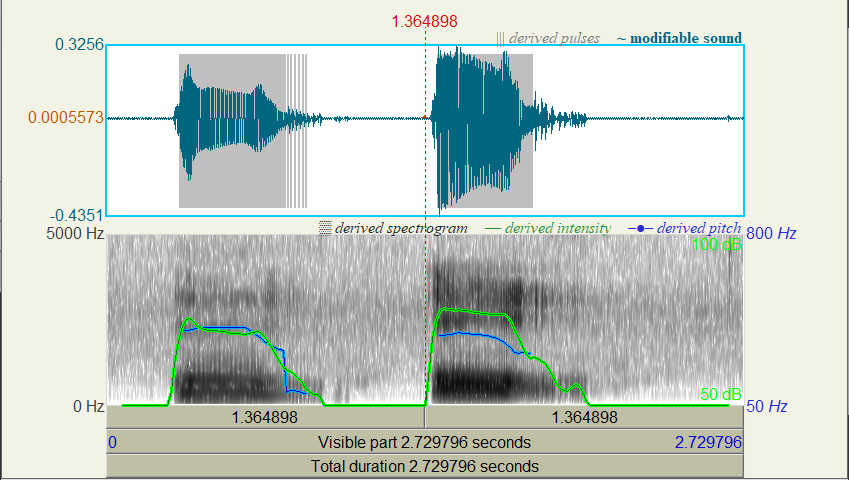
\includegraphics[width=0.65\linewidth]{img/u-o.png}
    \caption{Spectrogram of the /\textipa{u}/ and /\textipa{o}/ vowel sounds}\label{fig:u-o}
\end{figure}

It should be noted that the samples in
\cref{fig:halo,fig:hal'o,fig:halu,fig:hal'u} do not account for potential
allophonic changes in the syllable ``ha'' in the word ``Halo-Halo''. Here, we
simply assume that ``ha'' is pronounced identically in both duplications.

However,~\cite{KWF2015} indicates that ``Halo-Halo'' can be pronounced as
/\textipa{h'alo hal'o}/, with a glottal stop occurring between the glottal
fricative [\textipa{h}] and the open front unrounded vowel [\textipa{a}].
\Cref{fig:a-a'} illustrates both sounds in the spectrogram.

\begin{figure}
    \centering
    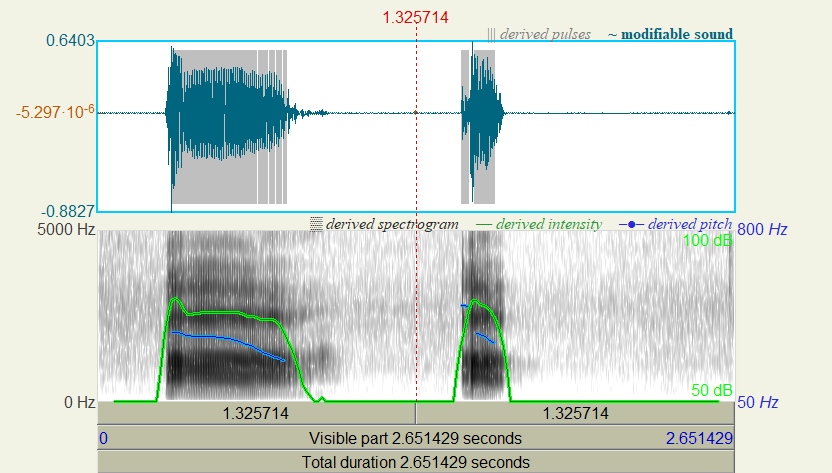
\includegraphics[width=0.65\linewidth]{img/a-a_.png}
    \caption{Spectrogram of the /\textipa{a}/ and /\textipa{'a}/ sounds}\label{fig:a-a'}
\end{figure}

The left spectrogram is the /\textipa{a}/ sound which we see is a continuous
sound that is slowly tapering off. While, the right is the /\textipa{'a}/ sound
which has an abrupt stop.

\subsection{Correct Pronunciation of ``Halo-Halo''}
Overall, we expect the spectrogram of ``Halo-Halo'' to display four distinct
phonetic sections. The first section ends abruptly due to a glottal stop. It is
followed by two syllables containing plain vowel sounds, and the final section
ends with a vowel accompanied by another glottal stop.

This pattern is observed in \cref{fig:correct}.

\begin{figure}
    \centering
    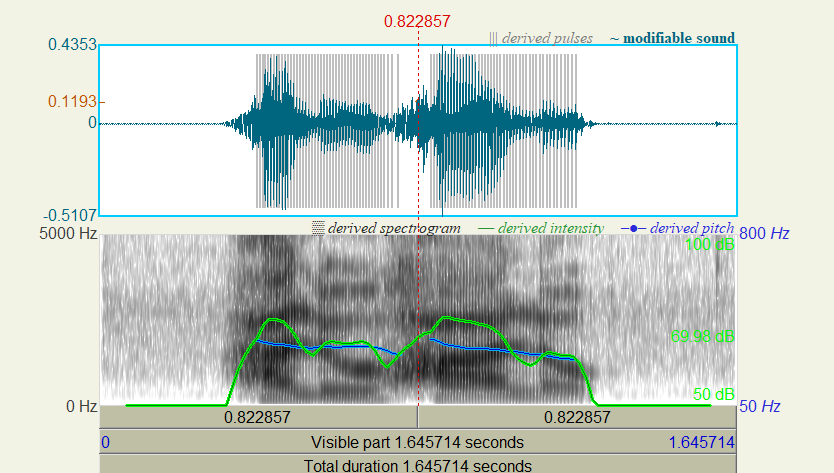
\includegraphics[width=0.65\linewidth]{img/correct.png}
    \caption{Spectrogram of the /\textipa{a}/ and /\textipa{'a}/ sounds}\label{fig:correct}
\end{figure}

\subsection{Conclusion}

Variations in possible pronunciations of ``Halo-Halo'' arises from the
widespread use of \emph{common spelling} (writing without diacritics) in most
Philippine contexts. The word's pronunciation can be clearly inferred when
using its \emph{diacritic orthography}: ``h\'alo-Hal\`o'', which indicates the
stressed syllables and glottal stops.

\section{Emotional Speech}

\bibliography{refs}
\bibliographystyle{alpha}
\end{document}